A partir de la revisi\'on bibliogr\'afica \cite{alvo2021,perumal2022,picarelli2020,vankootenniekerk2017,zhang2024} y de las caracter\'isticas del problema, se identificaron tres alternativas metodol\'ogicas. La primera es una metaheur\'istica Adaptive Large Neighborhood Search (ALNS) que construye y mejora iterativamente una soluci\'on factible mediante operadores de destrucci\'on y reparaci\'on, con buena escalabilidad a costa de no garantizar optimalidad. La segunda combina Set Partitioning, Generaci\'on de Columnas y cortes de Benders, representando cada jornada factible como una columna y verificando que las recargas sean compatibles con la infraestructura; evita un MILP monol\'itico de gran tama\~no, aunque su implementaci\'on es m\'as compleja.

La tercera, y la seleccionada por el grupo, es una descomposici\'on espaciotemporal, que agrupa los viajes por cercan\'ia a cada electroterminal y luego los divide en ventanas horarias superpuestas resueltas por horizonte rodante, transformando el problema en subproblemas E-VSP m\'as peque\~nos resolubles con MILP directo o, en ventanas complejas, con Set Partitioning y Benders. Su beneficio es hacer tratable la escala real de RED, a costa de la optimalidad global.

\section{Metodolog\'ia 1: Adaptive Large Neighborhood Search \label{sec:metodologia1}}

Una primera alternativa ser\'ia abordar el problema mediante una metaheur\'istica de tipo Adaptive Large Neighborhood Search (ALNS). Este enfoque no garantiza la soluci\'on \'optima, sino que construye una soluci\'on inicial factible y la mejora iterativamente mediante operadores de modificaci\'on, buscando minimizar buses utilizados, costos operacionales y desplazamientos sin pasajeros, explorando el espacio de soluciones de forma heur\'istica en lugar de con una formulaci\'on matem\'atica exacta. As\'i, sacrifica algo de optimalidad a cambio de eficiencia computacional.

Una soluci\'on corresponde a la asignaci\'on completa de viajes y decisiones de carga a cada bus (el conjunto de jornadas vigentes en un momento del algoritmo). El proceso parte de una regla simple (asignar los viajes en orden de horario al primer bus disponible que pueda ejecutarlos sin quedar sin bater\'ia, despachando uno nuevo si ninguno puede hacerlo). Sobre esta soluci\'on se aplican iterativamente un operador de destrucci\'on, que remueve viajes con mayor desplazamiento sin pasajeros o conflicto de carga, y uno de reparaci\'on, que reinserta esos viajes en la posici\'on de menor costo que preserve horarios, bater\'ia y capacidad de carga (agregando un bus nuevo solo si es necesario). La nueva soluci\'on se acepta si mejora la actual, y ocasionalmente aunque empeore, con probabilidad decreciente, para evitar quedar atrapado en una soluci\'on de baja calidad. El ciclo se repite hasta un criterio de t\'ermino, priorizando los operadores con mejores resultados recientes.

Esta metodolog\'ia ha sido aplicada con \'exito a problemas de estructura similar al nuestro: \citeA{wang2024} dise\~nan un ALNS para un problema con m\'ultiples electroterminales y restricciones de infraestructura de carga, con operadores de destrucci\'on y reparaci\'on adaptados al problema (por ejemplo, priorizar la remoci\'on de viajes con mayor holgura horaria, o reconstruir las jornadas de mayor costo promedio) y un mecanismo de aceptaci\'on tipo recocido simulado. En su experimento, el algoritmo alcanza una primera soluci\'on factible en 13,6 minutos y sigue mejor\'andola de forma consistente, demostrando que el enfoque genera soluciones de buena calidad en tiempos razonables pese a la alta complejidad combinatoria del problema conjunto de asignaci\'on y carga.

Los datos disponibles son consistentes con los supuestos de esta metodolog\'ia, ya que se tienen cinco electroterminales, validando el car\'acter multi-electroterminal del problema, y se dispone de la informaci\'on de capacidad de cargadores, par\'ametros de bater\'ia y tarifas necesaria para modelar las restricciones de carga. Dada la escala real del problema (417 rutas y 64.502 expediciones), una implementaci\'on completa probablemente se beneficiar\'ia de una descomposici\'on previa por zona o ventana horaria, siguiendo a \citeA{zhou2024}, quienes combinan un m\'etodo exacto para subproblemas peque\~nos con ALNS para la escala completa en la red de Singapur (m\'ultiples electroterminales y flota heterog\'enea).

\section{Metodolog\'ia 2: Set Partitioning con Generaci\'on de Columnas y Cortes de Benders \label{sec:metodologia2}}

Otra alternativa consiste en formular el problema mediante Set Partitioning y resolverlo utilizando Generaci\'on de Columnas, complementada con una verificaci\'on de los itinerarios de carga mediante cortes de Benders. Esta metodolog\'ia busca determinar la cantidad de buses el\'ectricos requerida y seleccionar un conjunto de jornadas que permita cubrir exactamente una vez todos los viajes entregados por la planificaci\'on, minimizando la cantidad de buses utilizados, los costos operacionales asociados y los desplazamientos sin pasajeros.

La metodolog\'ia se entiende como una con dos niveles de decisi\'on. En el primero se seleccionan las jornadas de buses mediante Set Partitioning y Generaci\'on de Columnas. En el segundo se verifica y programa el itinerario conjunto de carga.

Cada columna generada corresponde a una jornada completa propuesta para un bus, con sus secuencias de viajes, desplazamientos en vac\'io y periodos de espera, junto con la evoluci\'on de bater\'ia durante todo el recorrido (por ejemplo, salida del electroterminal, varios viajes consecutivos, una recarga y el retorno). Estas columnas deben ser individualmente factibles en horarios, energ\'ia y ubicaciones, pero no determinan la hora exacta ni el cargador a utilizar, ya que eso depende de la necesidad de carga conjunta de todos los buses.

Como visi\'on preliminar de la formulaci\'on, la principal variable de decisi\'on del problema maestro ser\'a binaria e indicar\'a si una determinada jornada factible es seleccionada o no:
\begin{equation}
Y_j = \begin{cases} 1 & \text{si se selecciona la jornada } j \\ 0 & \text{en caso contrario} \end{cases}
\label{eq:variabley}
\end{equation}

La restricci\'on fundamental de Set Partitioning exigir\'a que cada viaje programado pertenezca exactamente a una de las jornadas seleccionadas:
\begin{equation}
\sum_{j} a_{ij}\, Y_j = 1 \qquad \forall i
\label{eq:setpartitioning}
\end{equation}

Adicionalmente, el subproblema de carga deber\'a asegurar que las recargas programadas no superen simult\'aneamente la capacidad disponible de cada electroterminal, y por ende que las necesidades de carga e itinerarios creados sean posibles de cumplir con la capacidad conjunta de los cinco electroterminales.

El problema maestro selecciona la combinaci\'on de columnas de menor costo que cubre todos los viajes una vez. Dada la gran cantidad de jornadas posibles, la Generaci\'on de Columnas parte de un conjunto reducido y resuelve una versi\'on restringida del problema maestro; un subproblema busca nuevas columnas que mejoren la soluci\'on actual y las agrega solo si lo logran, repitiendo el procedimiento.

Una vez obtenida una soluci\'on candidata, un subproblema tipo Benders verifica si sus requerimientos de carga pueden satisfacerse con la infraestructura disponible en cada momento, determinando horarios, ubicaci\'on y duraci\'on de carga de cada bus. Aunque cada jornada sea factible individualmente, su combinaci\'on puede no serlo si excede la carga disponible en algún terminal; de detectarse esa infactibilidad, se genera un corte que se incorpora al problema maestro para evitar volver a seleccionar ese conjunto de columnas.

\textbf{Aspectos positivos:}
\begin{itemize}
\setlength{\itemsep}{1pt}
\item Descompone un problema de gran escala en componentes manejables, evitando resolver simult\'aneamente todas las decisiones de viajes y carga.
\item Set Partitioning representa de forma natural la operaci\'on de cada bus mediante jornadas completas (viajes, desplazamientos sin pasajeros, espera y evoluci\'on de bater\'ia).
\item La Generaci\'on de Columnas evita enumerar todas las jornadas factibles, generando solo las que contribuyen a mejorar la soluci\'on.
\item El subproblema tipo Benders separa las restricciones compartidas de carga, verificando compatibilidad con la infraestructura disponible.
\end{itemize}

\textbf{Aspectos negativos:}
\begin{itemize}
\setlength{\itemsep}{1pt}
\item Alta complejidad de implementaci\'on, pues exige coordinar iterativamente un problema maestro, un subproblema de columnas y un subproblema de factibilidad de carga.
\item Las restricciones compartidas entre buses (capacidad simult\'anea de cargadores) pueden provocar m\'ultiples iteraciones antes de una planificaci\'on globalmente factible.
\item Al trabajar inicialmente sobre la relajaci\'on lineal, obtener una soluci\'on entera puede requerir etapas adicionales, haciendo su desarrollo computacional m\'as exigente que un MILP directo.
\end{itemize}

\section{Metodolog\'ia Propuesta: Descomposici\'on Espaciotemporal \label{sec:metodologiapropuesta}}

La metodolog\'ia que proponemos consiste en descomponer el problema espacial y temporalmente. En lugar de optimizar simult\'aneamente todos los viajes de la red, se segmentan y agrupan en torno a los cinco electroterminales, considerando el lugar de inicio y t\'ermino de cada viaje, su distancia al electroterminal, los desplazamientos sin pasajeros (\emph{deadheads}) y su compatibilidad con otros viajes. Luego, cada bloque de recorridos por electroterminal se descompone en subproblemas por horas, cada uno resolviendo la asignaci\'on de viajes y el programa de carga para las paradas dentro de esa ventana.

Existe evidencia que respalda ambas descomposiciones; el desaf\'io est\'a en combinarlas. La descomposici\'on espacial es un principio cl\'asico en problemas VSP/VRP de gran escala, y consiste en agrupar primero los viajes por ubicaci\'on/terminal y luego resolver el ruteo de cada grupo por separado. \citeA{gao2024} utilizan esta idea en un MDVSP (multidep\'osito) similar al nuestro, asignando inicialmente los viajes a un dep\'osito, resolviendo el problema por dep\'osito y repitiendo el procedimiento tras ajustar el agrupamiento hasta obtener una soluci\'on satisfactoria; este enfoque es replicable a las electroterminales de nuestro problema.

La descomposici\'on temporal es m\'as dif\'icil, por lo complicado de unir soluciones que quedan atravesadas entre los l\'imites de los intervalos. \citeA{kim2023} muestran por qu\'e cortar el tiempo en bloques fijos es riesgoso, y proponen en cambio crear intervalos de tiempo superpuestos y resolver mediante un enfoque de horizonte rodante, iterando sobre una secuencia de intervalos superpuestos en vez de bloques disjuntos.

Para el desarrollo del m\'etodo proponemos estructurarlo en dos fases, cada una con su propio problema de optimizaci\'on.

\subsection{Fase 1: Asignaci\'on Espacial \label{sec:fase1}}

Se formula un problema de asignaci\'on de transporte con una variable binaria que indica si un viaje se asigna a un electroterminal (uno y solo uno por viaje). El costo se define por el \emph{deadhead} de ida m\'as el de vuelta al terminal, asignando el de menor costo (aproximado, pues el viaje podr\'ia encadenarse con otro antes de volver); la capacidad de cada terminal viene de \texttt{charging\_activities.csv}. El objetivo es minimizar el \emph{deadhead} total, balanceando la carga entre los cinco electroterminales. Este problema es resoluble como una LP de transporte relajada, muy r\'apida; como una asignaci\'on de una sola pasada puede alejarse del \'optimo, se busca modificar el agrupamiento, de ser necesario, y repetir el proceso hasta lograr una distribuci\'on m\'as equitativa.

\subsection{Fase 2: Descomposici\'on Temporal \label{sec:fase2}}

Dada una asignaci\'on por bloques de viajes para cada electroterminal, se corta el d\'ia en ventanas de tiempo superpuestas de 3 horas que avanzan de a 1 hora (0:00--3:00, 1:00--4:00, 2:00--5:00, \ldots). El avance de 1 hora asegura que el l\'imite izquierdo de cada ventana caiga en una hora exacta, coherente con la granularidad de los bloques tarifarios de \texttt{charging\_activities.csv}, y que la primera hora de cada ventana, cuya soluci\'on se fija definitivamente, coincida con el inicio de un bloque tarifario, mientras las dos horas restantes quedan como horizonte flexible que se reoptimiza en la siguiente iteraci\'on. El largo de 3 horas responde a que los buses demoran 105 minutos (1:45 hrs) en cargar, por lo que para fijar la primera hora el modelo debe poder ``ver hacia el futuro'' hasta que los buses terminen de cargar. Al resolver cada ventana, solo se fija la primera hora; las dos horas siguientes act\'uan como borrador que se reoptimiza en la iteraci\'on siguiente, con m\'as informaci\'on de los pr\'oximos viajes. El estado de cada bus (ubicaci\'on, nivel de bater\'ia) se transmite como condici\'on inicial a la siguiente ventana.

Cada subproblema de la Fase 2 es una instancia peque\~na de E-VSP, correspondiente a un electroterminal por una ventana horaria, la cual puede ser resuelta con MILP directo o mezclarse con la Metodolog\'ia 1 y resolverse mediante Set Partitioning + Generaci\'on de Columnas, dado que est\'a a una escala reducida y las columnas son manejables.

Como apoyo a la propuesta, se realiz\'o una prueba de la asignaci\'on espacial de las 64.502 expediciones de los d\'ias laborales.

\begin{figure}[htb]
	\begin{center}
	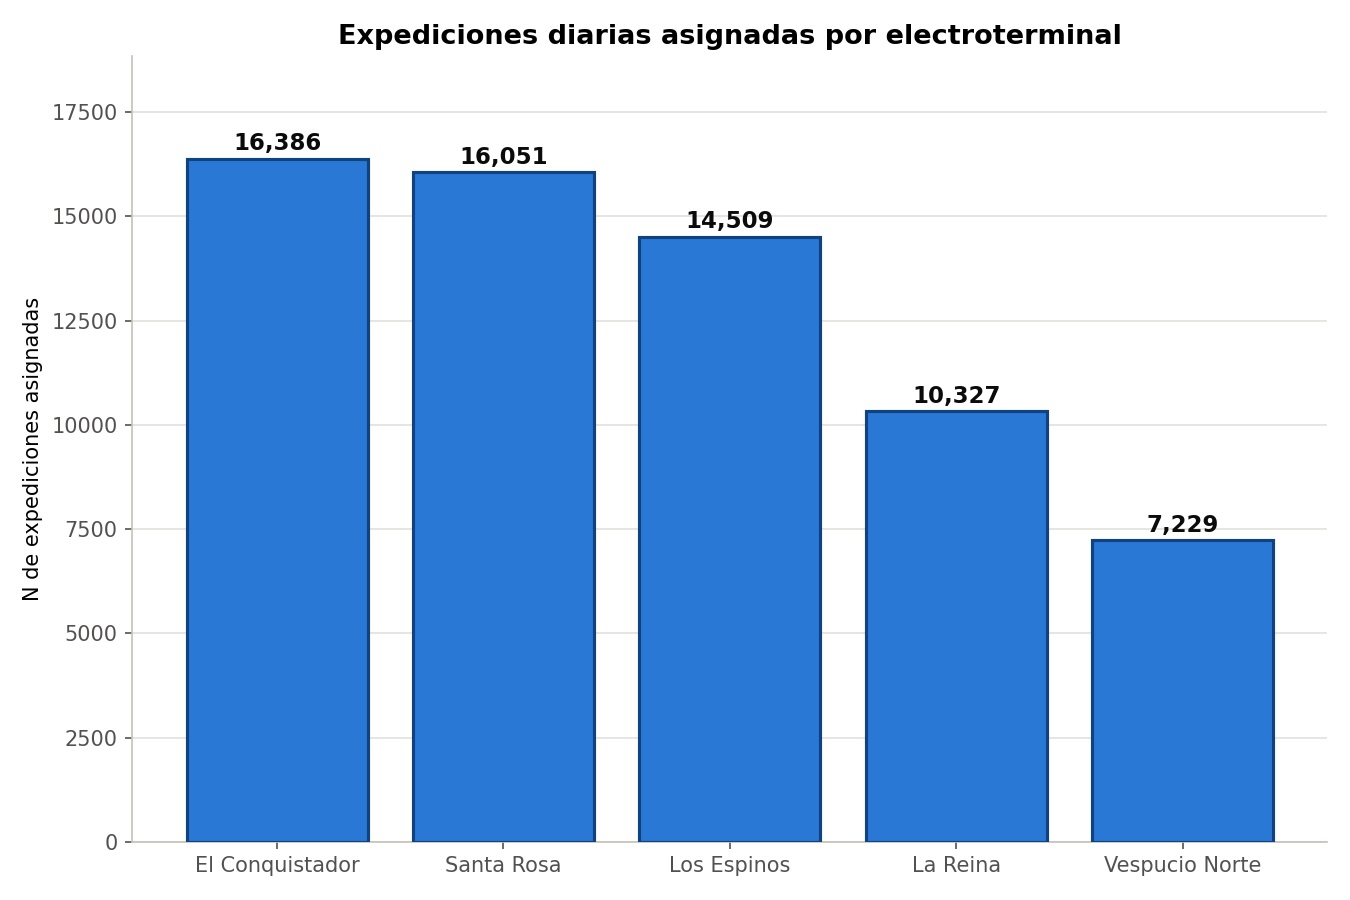
\includegraphics[width=0.55\textwidth]{./figures/expediciones_por_electroterminal.jpg}
	\caption[Expediciones diarias asignadas por electroterminal]{Expediciones diarias asignadas por electroterminal}
	\label{fig:expedicionesterminal}
	\end{center}
\end{figure}

Como se observa en la Figura \ref{fig:expedicionesterminal}, esta asignaci\'on distribuye las expediciones en cinco conjuntos de tama\~no reducido, transformando el problema completo en cinco problemas menores. Sin embargo, no asegura una asignaci\'on \'optima y puede restringir la concatenaci\'on de expediciones \'optimas, por lo que debe validarse y, de ser necesario, ajustar el criterio de asignaci\'on.

\textbf{Aspectos positivos:}
\begin{itemize}
\setlength{\itemsep}{1pt}
\item Reduce el problema de 64.502 expediciones / 5 electroterminales / 1 d\'ia a m\'ultiples subproblemas manejables, cada uno resoluble de forma exacta.
\item El uso de tarifas horarias encaja bien con la descomposici\'on temporal, ya que cada ventana sabe en qu\'e bloque de tarifas est\'a.
\item Puede integrarse con la Metodolog\'ia 2, ya que las ventanas de mayor complejidad (por ejemplo, las que calcen con horarios peak) pueden resolverse con Generaci\'on de Columnas y cortes de Benders.
\end{itemize}

\textbf{Aspectos negativos:}
\begin{itemize}
\setlength{\itemsep}{1pt}
\item Se pierde la garant\'ia de optimalidad global, ya que una mala asignaci\'on en la Fase 1 o una decisi\'on sub\'optima en la Fase 2 no se corrige salvo que se agregue un paso de reparaci\'on.
\item La calidad depende fuertemente del tama\~no de ventana, pues ventanas muy cortas empeoran la calidad, y muy largas devuelven el problema a lo original.
\item Alta complejidad de dise\~no, especialmente al decidir qu\'e informaci\'on del futuro pasar a cada subproblema para evitar decisiones que resulten infactibles m\'as adelante.
\end{itemize}

Dada esta complejidad, se planea una implementaci\'on progresiva, comenzando con versiones simplificadas del problema e incorporando gradualmente las restricciones hasta la formulaci\'on completa. Como estrategia alternativa, si la metodolog\'ia resulta demasiado exigente computacionalmente, se propone sacrificar la descomposici\'on temporal y centrarse principalmente en la asignaci\'on espacial de los viajes.
